\subsection{Trackpy (CuPy)}

When profiling the Trackpy code, the functions \texttt{fourier\_gaussian}, \texttt{uniform\_filter1d} and \texttt{correlate1d} from \texttt{SciPy} took a considerable amount of time.
For this reason, Trackpy's code was altered to use the \texttt{CuPy} library instead of \texttt{SciPy} for these operations.
This aimed to exploit the GPU for faster computation.

\subsubsection{Algorithm}

The algorithm is the same as Trackpy's, with some extra steps required to transfer the various arrays to/from GPU memory.
These transfers were reduced to the minimum, to reduce the overhead as much as possible.

\subsubsection{Evaluation}

Figure~\ref{fig:locate:trackpy-cupy} shows the result, which for unknown reasons is slightly worse than Trackpy's, at 79\% of identified bubbles.
The algorithm is however faster, running at 7 FPS, but still extremely far from the target.

\begin{figure}
	\centerline{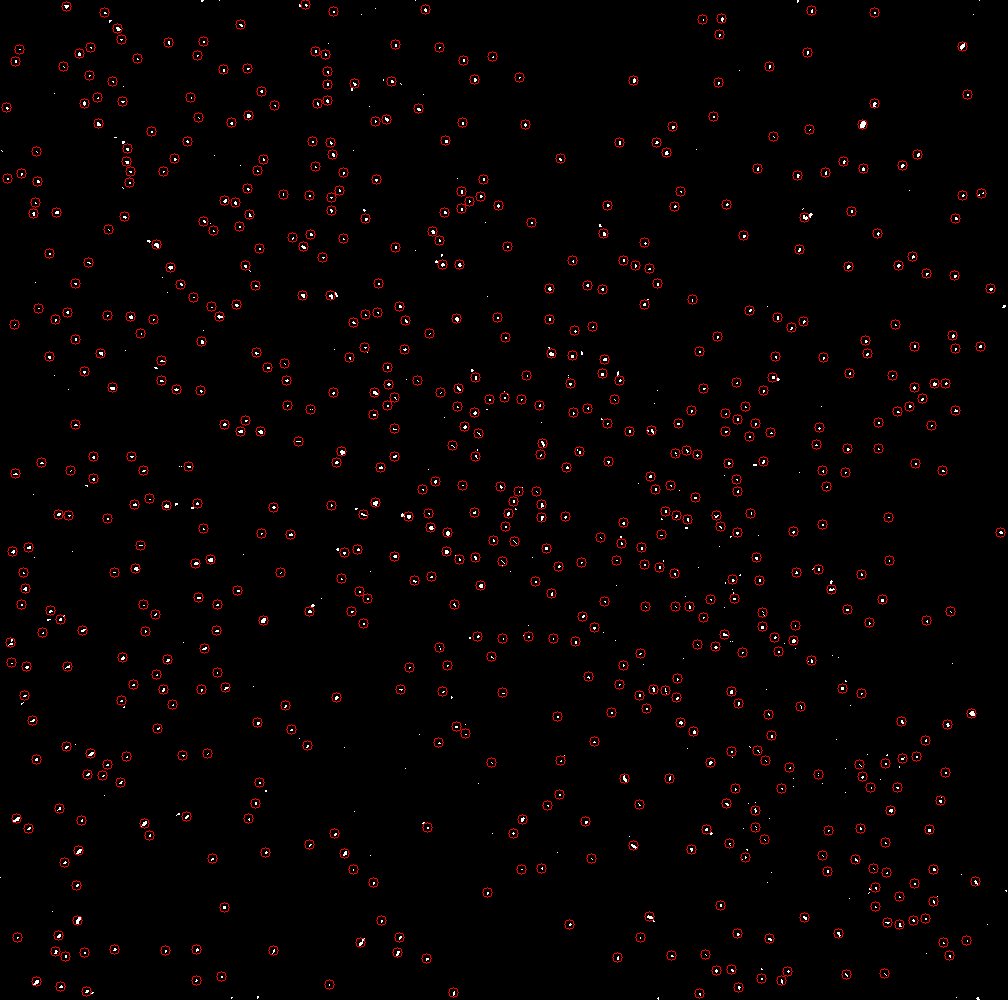
\includegraphics[width=\locateimgsize]{images/locate/cuda-trackpy.png}}
	\caption{\centering Trackpy with CuPy's result}
	\label{fig:locate:trackpy-cupy}
\end{figure}
